\documentclass[compress]{beamer}

\usepackage[utf8]{inputenc}
\usepackage{tikz}
\usepackage{amssymb}
\usepackage{listings}
\usepackage{algorithm}
\usepackage{tikz}
\usetikzlibrary {automata,positioning}
\usepackage[style=authortitle, backend=biber]{biblatex} %Imports biblatex package
\addbibresource{Citations.bib}

\usepackage[export]{adjustbox}


%___________________________________________________
% LST

\lstset{frame=tb,
  basicstyle=\small\ttfamily, % Global Code Style
  captionpos=b, % Position of the Caption (t for top, b for bottom)
  extendedchars=true, % Allows 256 instead of 128 ASCII characters
  tabsize=2, % number of spaces indented when discovering a tab 
  columns=fixed, % make all characters equal width
  keepspaces=true, % does not ignore spaces to fit width, convert tabs to spaces
  showstringspaces=false, % lets spaces in strings appear as real spaces
  breaklines=true, % wrap lines if they don't fit
  frame=trbl, % draw a frame at the top, right, left and bottom of the listing
  frameround=tttt, % make the frame round at all four corners
  framesep=4pt, % quarter circle size of the round corners
  %numbers=left, % show line numbers at the left
  %numberstyle=\tiny\ttfamily, % style of the line numbers
  morekeywords={True},
  keywordstyle=\color{RubineRed}, % style of keywords
  stringstyle=\color{Orchid}, % style of strings
}
% Types

\setbeamertemplate{navigation symbols}{}

\definecolor{ppurple}{rgb}{0.71,0.13,0.71}
\definecolor{pgreen}{rgb}{0,0.5,0}
\definecolor{pred}{rgb}{0.9,0,0}
\definecolor{pgrey}{rgb}{0.46,0.45,0.48}

\lstdefinelanguage{SMV} {
  morekeywords={VAR, IVAR, MODULE, ASSIGN, next, init, INIT, DEFINE, TRANS,
  LTLSPEC, CTLSPEC, case, esac
  }
}

\lstset{language=SMV,
  showspaces=false,
  showtabs=false,
  breaklines=true,
  showstringspaces=false,
  breakatwhitespace=true,
  commentstyle=\color{pgreen},
  keywordstyle=\color{ppurple},
  stringstyle=\color{pred},
  basicstyle=\small\ttfamily,
  moredelim=[il][\textcolor{pgrey}]{\$\$},
  moredelim=[is][\textcolor{pgrey}]{\%\%}{\%\%}
}
\usetheme[navigation]{UMONS}
\begin{document}
%\usetheme[navigation, no-subsection, no-totalframenumber]{UMONS}

\newcommand{\IR}{\mathbb{R}}

\title[NuXmv Tool presentation]{Tool presentation}
\subtitle{NuXmv}
\author[K.William \and B.Maxime]{
  Karpinski William 
  \and
  Bartha Maxime
}

\institute[]{%
  Computer Sciences department\\
  University of Mons
  \\[2ex]
  \includegraphics[height=4ex]{images/logoumons.jpg}\hspace{2em}%
  \raisebox{-1ex}{\includegraphics[height=6ex]{images/logofs.jpg}}
}

\begin{frame}[plain, noframenumbering]
  \maketitle
\end{frame}

\begin{frame}
  \frametitle{Outline}
  \tableofcontents
\end{frame}
\AtBeginSection[]
  {
     \begin{frame}<beamer>
     \frametitle{Plan}
     \tableofcontents[currentsection]
     \end{frame}
  }


\section{Introduction}

\begin{frame}
  \frametitle{Introduction}

\begin{figure}
  \begin{center}
    \includegraphics[width=0.80\textwidth]{images/Trans.png}
  \end{center}
\end{figure}


  Released in February 2014, nuXmv is a model checker based on NuSMV which appeared in 1999 (hence the logo)
\end{frame}

\begin{frame}
  \frametitle{Interface}

  \noindent\begin{minipage}{0.5\textwidth}% adapt widths of minipages to your needs
  \includegraphics[width=\textwidth,left]{images/Consol.png} 
  \end{minipage}%
  \hfill%
  \begin{minipage}{0.45\textwidth}\raggedright
    Even thought recent studies\footnotemark ~  have looked into formalizing a graphical user interface for nuXmv, it is a command line tool. 
  \end{minipage}
  \footnotetext[1]{\cite{inproceedings}}
\end{frame}


\begin{frame}[fragile]
  \frametitle{Models definition}
  \begin{itemize}
    \item SMV file
      \begin{itemize}
        \item Symbolic representation of a Kripke Structure (TS without labels on actions)
      \end{itemize}
  \end{itemize}

\begin{lstlisting}[language=SMV]
  MODULE main
    VAR
      s0 : boolean;
    INIT
      !s0;
    TRANS
      s0 -> next(!s0);
  \end{lstlisting}

\end{frame}





\section{Model Checking}
\begin{frame}
\frametitle{Model Checking}
  Finite-state systems
  \begin{itemize}
    \item BDD-based algorithm
    \item SAT-based algorithms
      \begin{itemize}
        \item Bounded Model Checking (BMC)
        \item K-Liveness
      \end{itemize}
  \end{itemize}
\end{frame}

\begin{frame}
\frametitle{Algorithms}
\begin{itemize}
  \item BDD-based algorithm
  \begin{itemize}
    \item LTL and CTL
    \item Convert formula into a BDD, with propositional logic
    \item Heritated from $nuSMV$
    \item check\_ltlspec, check\_ctlspec
  \end{itemize}
\end{itemize}
\end{frame}

\begin{frame}
\frametitle{Algorithms}
    \begin{itemize}
        \item SAT-based algorithms 
        \begin{itemize}
          \item LTL only
        \end{itemize}
      \item BMC
        \begin{itemize}
          \item Try to find a counter example in a bound $k$
          \item $k$ chosen by default by $nuXmv$
          \item check\_ltlspec\_bmc
        \end{itemize}
      \item K-liveness
      \begin{itemize}
        \item Try to find a counter example using invariant induction proof
        \item Implement IC3
        \item check\_ltlspec\_ic3
        
      \end{itemize} 

    \end{itemize}

\end{frame}

\begin{frame}
  \frametitle{Model Checking}
    \begin{figure}
    \begin{center}
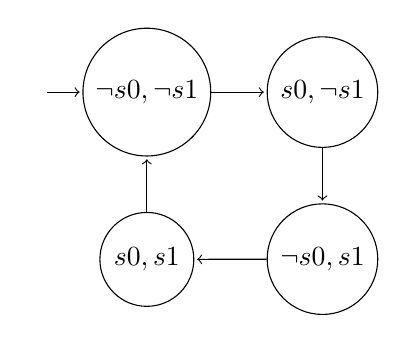
\begin{tikzpicture}[shorten >=1pt,node distance=20pt,auto,initial text=]

  \node[state,initial]  (q_0)                {$\neg s0,\neg s1$};
  \node[state]          (q_1) [right=of q_0] {$s0,\neg s1$};
  \node[state]          (q_2) [below=of q_1] {$\neg s0,s1$};
  \node[state]          (q_3) [below=of q_0] {$s0,s1$};

  \path[->] (q_0) edge node {} (q_1)
            (q_1) edge node {} (q_2)
            (q_2) edge node {} (q_3)
            (q_3) edge node {} (q_0);
\end{tikzpicture}
    \end{center}
\end{figure}
\begin{itemize}
  \item $\phi_1 := \square (\diamond (s0\land s1))$
\end{itemize}
    \begin{figure}
      \begin{center}
        \includegraphics[width=0.75\textwidth]{images/bdd_phi_1.png}
      \end{center}
    \end{figure}
    

\end{frame}


\begin{frame}
  
  \frametitle{Model Checking}
  
  \begin{itemize}
    \item go\_bmc : setup model for SAT-model checking
    \item BMC : does not provide a definitive answer
  \end{itemize}

 \begin{figure}[!htb]
    \centering
    \begin{minipage}{.4\textwidth}
        \centering
        \includegraphics[width=0.5\textheight]{images/bmc_phi_1.png}
        \caption{BMC}
    \end{minipage}%
    \begin{minipage}{0.4\textwidth}
        \centering
        \includegraphics[width=0.5\textheight]{images/IC3_phi_1.png}
        \caption{K-liveness}
    \end{minipage}
\end{figure} 
\end{frame}

\begin{frame}
  \frametitle{Model Checking}
    \begin{figure}
    \begin{center}
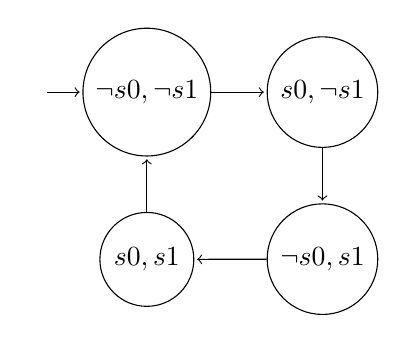
\begin{tikzpicture}[shorten >=1pt,node distance=20pt,auto,initial text=]

  \node[state,initial]  (q_0)                {$\neg s0,\neg s1$};
  \node[state]          (q_1) [right=of q_0] {$s0,\neg s1$};
  \node[state]          (q_2) [below=of q_1] {$\neg s0,s1$};
  \node[state]          (q_3) [below=of q_0] {$s0,s1$};

  \path[->] (q_0) edge node {} (q_1)
            (q_1) edge node {} (q_2)
            (q_2) edge node {} (q_3)
            (q_3) edge node {} (q_0);
\end{tikzpicture}
    \end{center}
\end{figure}
\begin{itemize}
  \item $\phi_2 := \diamond (\square (\neg s0 \land \neg s1))$
\end{itemize}
    
\end{frame}

\begin{frame}
  \frametitle{Model Checking}
    \begin{figure}
      \begin{center}
        \includegraphics[width=0.5\textwidth]{images/bdd_phi_2.png}
      \end{center}
      \caption{BDD-algorithm}
    \end{figure}
\end{frame}
\begin{frame}

  \frametitle{Model Checking}
 \begin{figure}[!htb]
    \centering
    \begin{minipage}{.4\textwidth}
        \centering
        \includegraphics[width=0.5\textheight]{images/bmc_phi_2.png}
        \caption{BMC}
    \end{minipage}%
    \begin{minipage}{0.4\textwidth}
        \centering
        \includegraphics[width=0.5\textheight]{images/IC3_phi_2.png}
        \caption{K-liveness}
    \end{minipage}
    \end{figure}
\end{frame}

\begin{frame}
  \frametitle{Model Checking}
  Infinite-state Systems
  \begin{itemize}
    \item Reals and integers implemented
    \item SMT-Based algorithms and abstraction
      \begin{itemize}
        \item BMC, K-liveness
      \end{itemize}
 \end{itemize}
\end{frame}
  % BDD-Based model checking
  %
  %
  % SAT model checking
  %   BMC : Bounded model checking
  %   K-liveness
  %   IC3
  %
  %
  % BMC idea:
  %   SATisfiabilité pour CNF en temps poly
  %   GOAL: étant donné une formule et un time bound k
  %   Construire formule propositionnelle satisfiable ssi valid sur un chemin 
  %   de longueur k si cest le cas alors on a un contre exemple si pas alors
  %   la formule est good
  %
  % IC3 & k-liveness
  %   Solve verification problem avec plein de mini SAT queries
  %
  %
  % SAT can DO ALL LTL, en principe TOUT CTL mais research pour retirer
  % quantificateurs
  %
  % SAT better when at finding errors fast and giving counter examples
  % BDD better proving no errors
  %

\section{Examples}


\printbibliography

\end{document}
%%% Local Variables: 
%%% mode: latex
%%% TeX-master: t
%%% ispell-local-dictionary: "fr"
%%% End: 

